\chapter{Results}

\section{Original Data}

Here we will explore the results of different classifiers and active learning strategies on the original data. The original data consisted of data shown previously in Figure \ref{fig:original_english_counts} and discretely in Table \ref{tab:en_data_counts} in Appendix \ref{app:attachments}. 

\subsection{Active Learning with PWC and RBF Kernel}

In Figure \ref{fig:plot_all_results_rbf} we have the train and test errors for four different active learning sampling strategies and we can see that xPAL and PAL both perform relatively well before starting to over-fit the training data. We reviewed the resulting error data and xPAL outperformed PAL by about 1.5\%. However, xPAL has much faster running time compared to PAL.

We weren't satisfied with the testing error which leveled out to about 70\% for each sampling strategy. PAL and xPAL were able to rapidly reduce the testing error early on in the training process while random selection and QBC weren't able to determine the data with the highest information gain. 

\begin{figure}[ht]
  \centering
  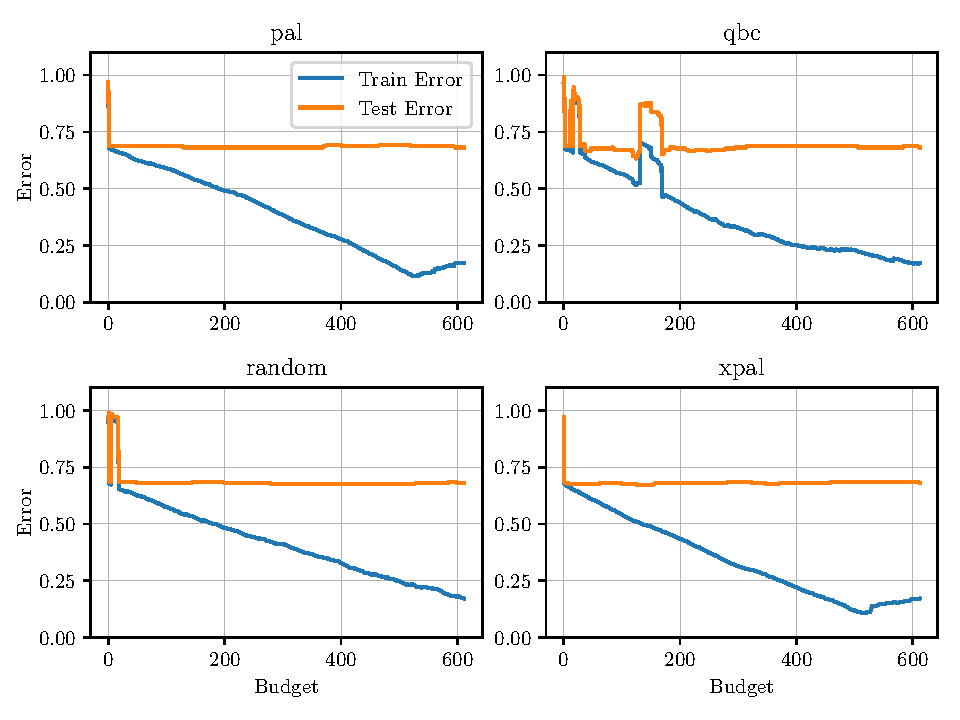
\includegraphics[width=\textwidth]{../img/plot_all_results_rbf.pdf}
  \caption{Train and test error using different query strategies and RBF kernel for the PWC classifier.}
  \label{fig:plot_all_results_rbf}
\end{figure}

\subsection{Active Learning with PWC and Cosine Kernel}

In Figure \ref{fig:plot_all_results_cosine} we have the and test errors for the same four different active learning sampling strategies and tested on the same data except instead of using the RBF kernel the Cosine kernel was used. We found that using the Cosine kernel reduced the training error across the board by roughly 17\%.  

\begin{figure}[ht]
  \centering
  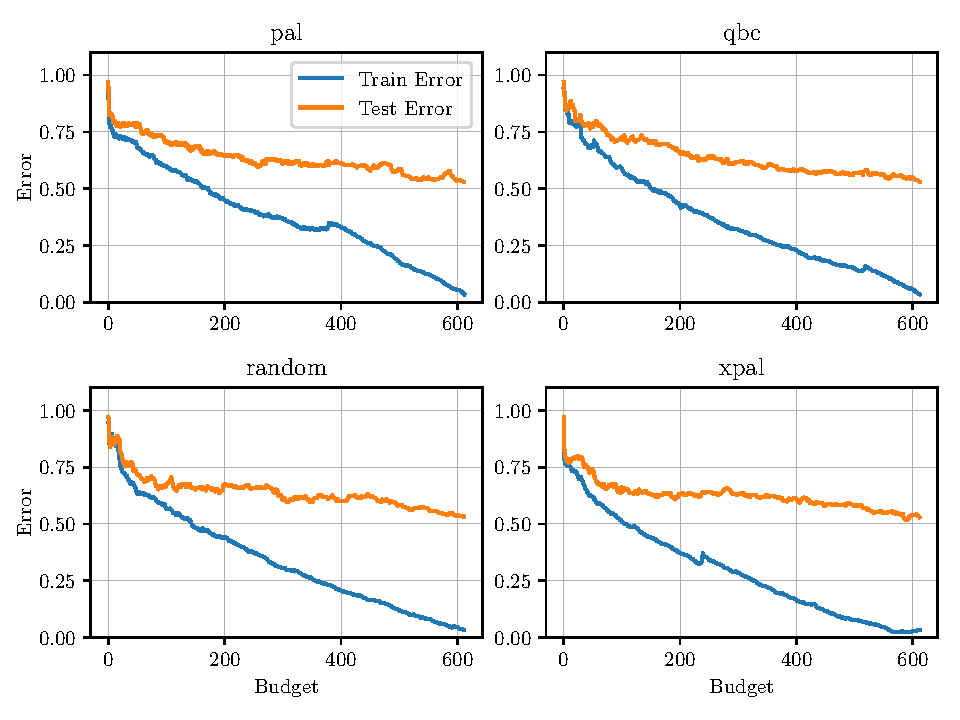
\includegraphics[width=\textwidth]{../img/plot_all_results_cosine.pdf}
  \caption{Train and test error using different query strategies and Cosine kernel for the PWC classifier.}
  \label{fig:plot_all_results_cosine}
\end{figure}


In Figure \ref{fig:plot_all_results_cosine} PAL and xPAL were able to reduce the training error, by about 20\% and 25\% respectively, early in the training process compared to random selection and QBC.

\subsection{Scikit-Learn Classifier Evaluation}

We also decided to try out the boilerplate classifiers from Scikit-Learn to compare performances. Again we used the original data with the same TF-IDF vectorizer as used with the previous active learning models to stay consistent. Cross validation was also used here but was not used in the previous sections. We decided to use the Cosine kernel when using LinearSVC as we learned that the performance increased in comparison to the RBF kernel when using PWC. The results for a variety of different classifiers are shown in Figure \ref{fig:explore_classifiers}. In the box-plot, the whiskers extend from the box to the furthest data points that are within 1.5 times the inter-quartile range (IQR) of the box. Any data points that are beyond the whiskers are considered outliers and are plotted as individual points or symbols (diamonds) as seen in Figure \ref{fig:explore_classifiers}.

\begin{figure}[ht]
  \centering
  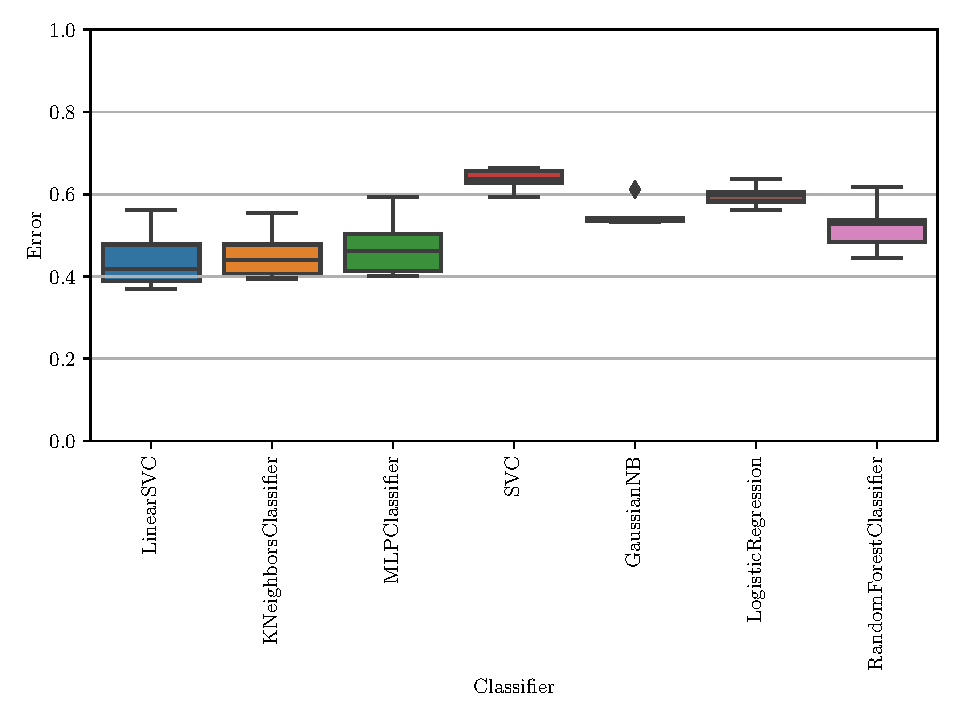
\includegraphics[width=\textwidth]{../img/plot_explore_classifiers.pdf}
  \caption{Performance of standard Scikit-Learn classifiers without optimization.}
  \label{fig:explore_classifiers}
\end{figure}

The LinearSVC classifier performed rather well compared to most other classifiers and it is a fast running algorithm even with data that has a large feature set. We decided to look further into LinearSVC and create a few models to evaluate its performance. We created three models, the first was a boilerplate LinearSVC with no argument modifications, the second model used the class weights parameter set to 'balanced'. The 'balanced' mode uses the values of y to automatically adjust weights inversely proportional to class frequencies in the input data as $n\_samples / (n\_classes * np.bincount(y))$. For the third test we created a dictionary of weights for each class using the Cosine Decay function. The weights for each category ranged from 0.1 to 1.0 where the most frequent classes had smaller weights. The results are shown in Table \ref{tab:lsvc_models}.


\begin{table}[h]
\centering
\begin{tabular}{|l|l|}
\hline
{} & \textbf{Error} \\
\hline
Balanced Weights & 0.441 \\
\hline
Boilerplate & 0.406 \\
\hline
Cosine Decay Weights & 0.392 \\
\hline
\end{tabular}
\caption{Error for three different LinearSVC models.}
\label{tab:lsvc_models}
\end{table}


\section{Original and Additional Data}